\chapter{Theory}
\label{ch:chapter2}
Following is a brief introduction to some of the aspects that affects the solution, and should be among the things considered when developing a commercial application.
\subsection{Camera}
The camera specifications and performance directly affects the results. It is the source of input data for the machine vision software, and it may also be the output, which will be the case when the PTZ\footnote{PTZ, pan- tilt and zoom functionality to translate the image captured by a camera. Common in dome-type CCTV cameras.} is controlled by the software.

Some cameras support extra applications that run in their operating system, which can for example track moving objects and "fence" an area so that any objects who enter a region of interest, will raise an alarm.
Embedded systems which can be found in commercial CCTV cameras are commonly resource-constrained in terms of CPU and RAM, and this suggests that some complex software applications should be executed on a stand-alone computer.

\subsubsection{Resolution and Field of view}
Resolution and field of view are related such that an increased field of view leads to a lower amount of pixels available to distinguish objects. Modern image sensors come with capabilities of capturing 1920x1080 pixel images, whilst older image sensors may capture 320x240 pixel images.
The field of view is a function of the optical objective as well as the size of the image sensor, and their distances in relation to each other.

\subsubsection{Pan, Tilt and Zoom}
Many modern CCTV cameras come with motors that can pan and tilt the camera, as well as optical and digital zoom functionality. Their ability to pan, tilt and zoom have uses for scanning a large area, as well as investigating small areas in detail.
The speed and accuracy of which the pan, tilt and zoom can be manipulated may be of importance in some applications.

\subsubsection{Focus}
If light from an object converges as much as possible, it is considered in focus. Would the light rather diverge, it is considered out of focus. This leads to blurring of the object or scene in question.
Many cameras come with automatic focus that will try to adjust the focus so that a target object becomes in focus. The focus is then controlled by either an ultrasonic motor or a stepper motor.

\subsubsection{Aperture}
The aperture is the opening in a camera objective which determines how much light enters the camera, and it is also a factor that can determine the focus range of a camera. An open aperture leads to larger amounts of light and thus works better in low-light conditions, but the depth of field gets smaller. See figure \ref{aperture_dof} for how depth of field relates to the aperture size. The amount of light that enters and hits the image sensor also determines how long the aperture should be kept open before a picture is fully captured, and less light means that it will need to stay open longer, which in turn leads to motion blur if an object is in motion.
Many cameras come with automatic aperture control, that will try to adjust the aperture opening and shutter speed so that the picture does not get too bright or too dark. Axis Communications have introduced a more precise aperture control to some cameras, which they call "P-iris", claimed to provide improvements to contrast, clarity, resolution and depth of field beyond other methods of aperture control.

\begin{figure}[ht]
    \centering
    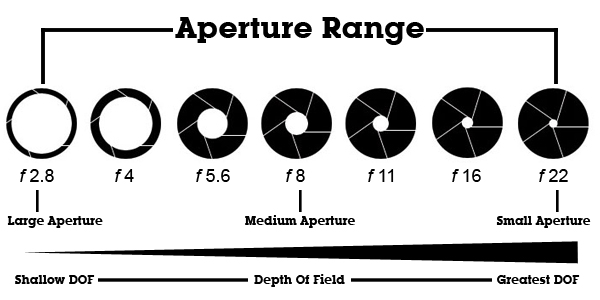
\includegraphics[width=0.8\textwidth]{aperture_dof.jpg}
    \caption{Aperture versus depth of field. Source: Online \citet{aperturedof15}}
    \label{fig:aperture_dof}
\end{figure}
\FloatBarrier

\subsubsection{Frame Rate}
The frequency of consecutive image frames is expressed in frames per second. Video displays motion through the constant change of image frames, and the human visual system perceives this as motion.
Capturing at a given frame rate requires the aperture, image sensor and the operating system of a digital camera to perform the job of capturing, processing and transmitting at the rate required.
A large amount of frames per second requires a multiple of the image resolution of bandwidth to transfer the images to a viewer, which means that the most direct way of reducing data transmission requirements is by reducing frames per second. When it comes to CCTV cameras for surveillance, frame rate of stored movies are reduced to allow for longer storage of the video material.
Higher frame rate gives perceived smoother motion in the video, and it also allows us to slow down actions and investigate them in detail.
The frame rate of a normal CCTV camera may be 25 FPS, a high-definition movie may be 60 FPS while high-speed cameras capture several thousands of frames per second.

\subsubsection{Image Quality}
The quality of an image is related to the quality of the optics, quality of the image sensor and amount of light available at a scene, as well as any video codec used to compress the image, in addition to other factors.
Modern image sensors can also adjust the sensitivity of the sensor so that previously dark scenes look brighter, at the cost of increased pixel noise.
A full overview over the factors that affect image quality can be found at \citep{imatest15}.

\subsubsection{Camera Interface}
Which interface that is supported for transferring images is an important factor to consider, and the focus can be to reduce cost or increase performance. The optimal interface depends on the application.
Some of the most used interfaces today includes USB, SDI and Ethernet. It is also possible to find CCTV cameras that rely on Wi-Fi, but these are prone to intermittent frame drops if environmental conditions blocks the signal.

\subsection{Data transmission}
A function of the camera hardware and operating system, the camera interface and path of transmission as well as any processing on the way, several aspects will affect data transmission from the image sensor to the screen. An unfortunate side-effect of data transmission is that an image lags after the actual event got captured, and we commonly call this for latency. The way a video signal propagates from one place to another makes this an important parameter in the selection of a camera system. At each end of the transmission line, compression and decompression may take place.

\paragraph{Analog}
Analog video transmission relies on a continuous voltage range. A weak signal is susceptible to electronic interference. The analog signal is modulated on top of a carrier frequency using RF modulation, which is then transferred over a physical medium. The medium have major implications on the amount of interference the signal picks up. Coaxial cables are just one of the many mediums that can be used, including broadcasting over a VHF\footnote{VHF, Very high frequency is a designation for electromagnetic waves in the range from 30 MHz to 300 MHz.} or UHF\footnote{UHF, Ultra high frequency is a designation for electromagnetic waves in the range from 300 MHz to 3 GHz.} carrier.
\paragraph{Digital - SDI family}
A family of serial digital interface standards defined by the SMPTE in 1989 \citep{poynton03} is another method to transfer video. This family of standard is not widely used in consumer electronics, as licensing agreements restricts its use. Usually used to transfer uncompressed and unencrypted digital video signals, they can also be used for packetized data. The physical medium can be of copper coaxial cables with BNC connectors and 75 ohms impedance for a max run length of typically 100 meters when used with HD video, or it can be fiber optics only limited by the maximum fiber length and repeaters. The quality of cabling and termination is important to ensure max range. \citet{wikisdi15}

SMPTE 292M is one of these standards, common name is HD-SDI and it was introduced in 1998. Its theoretical bitrate is 1.485 Gigabit per second, and it can transfer up to 1080i images through coaxial cables.

Since SDI uses a dedicated coaxial cable, there is no network congestion.

\paragraph{Digital - IP}
Another digital method uses the Internet Protocol to transfer video as packets. This provides great flexibility  and range of the video signal, at the cost of reliability and risk of packet loss. Its task is to deliver packets from a source host to a destination based on the IP addresses in its packet header. The physical medium is commonly twisted-pair cable for cheap and reliable end-node communication, fiber optical cable for long-range high-bandwidth connections, or wireless RF where the data is modulated on a carrier wave of 2.4 GHz or 5 GHz.

The complexity of IP communication is reduced to layers that provide a specific task, and a conceptual model known as the OSI model shows this. The OSI model can be seen illustrated in figure \ref{fig:osi_model_overview}. Since the packets are moved through intermediate routers and switches, a packet can travel around the world almost instantly, but all packet handling and propagation of the signal will incur delay.

For local networks, the complexity of IP communication, wrapping of packets with destination address and other features of IP communication translates to delay between two host applications.

Video compression using a video codec is used to allow image data to be reduced in size to not congest the network, and the video codecs available for a given IP camera varies.

IP communication hardware is cheap and abundant, flexible and dynamic. Network congestion may lead to packet loss.

\begin{figure}[ht]
    \centering
    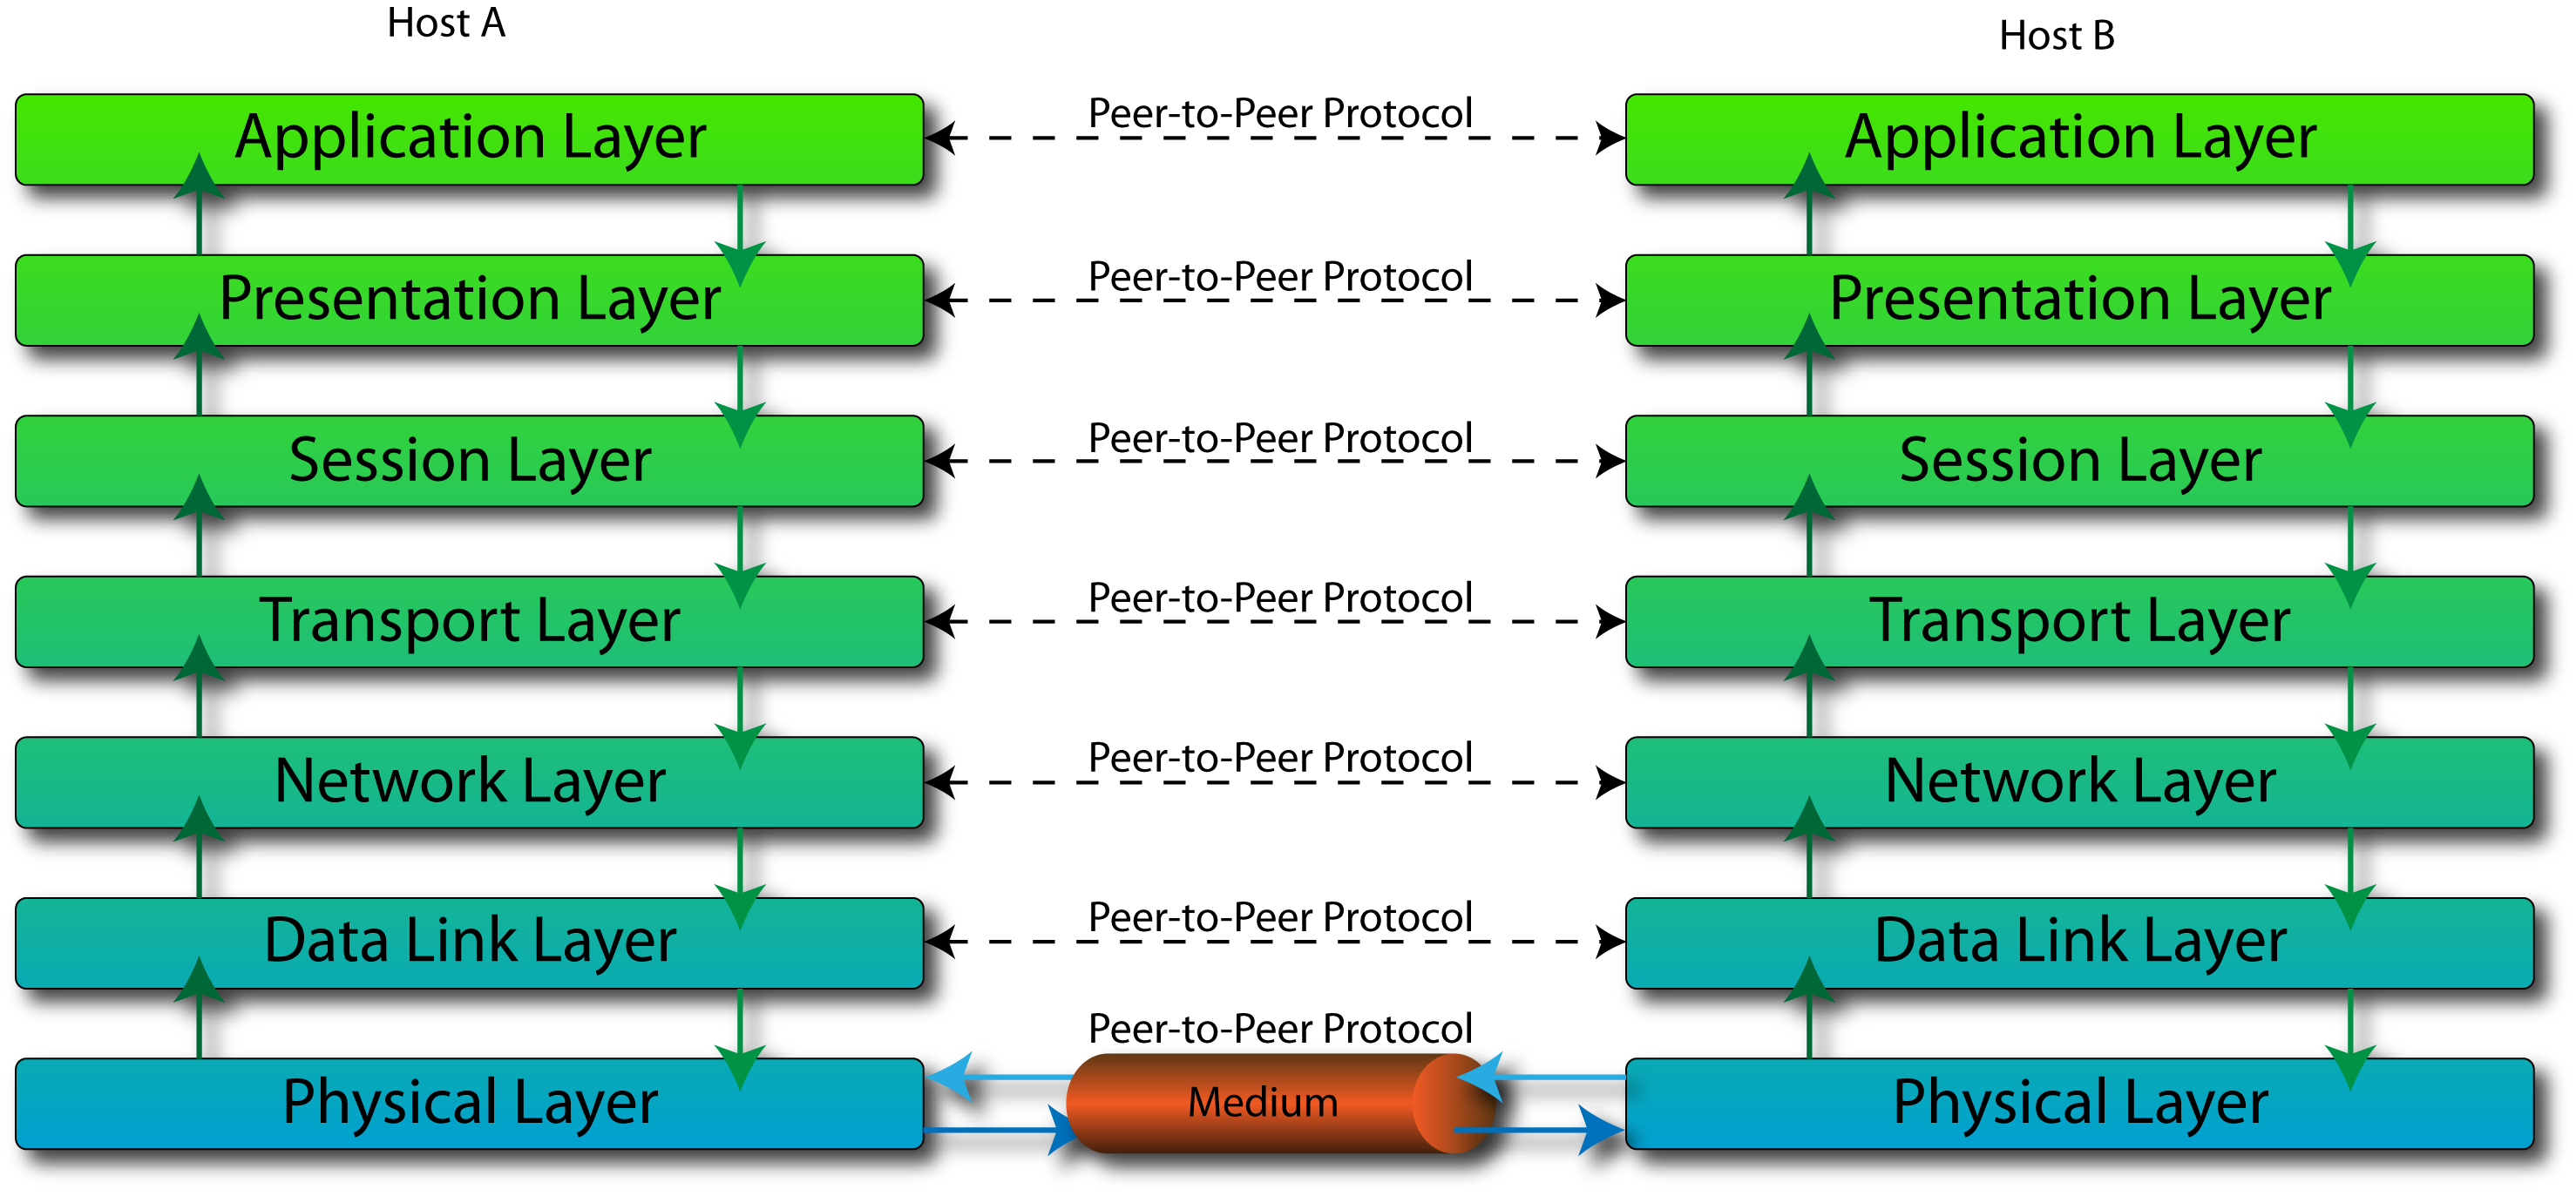
\includegraphics[width=1.0\textwidth]{osi_model_overview.png}
    \caption{The OSI model and communication from host A to B. Source: \citet{osi15}}
    \label{fig:osi_model_overview}
\end{figure}
\FloatBarrier

\subsection{Video compression}
A video codec is used to compress image data for transmission, and decompress it when it has arrived at its destination. It is also used for storing video on a computer. Compression is typically lossy, which means that data is removed on purpose to reduce the need for storage. We can divide video codecs into two groups, one group relying on intraframe- and the other on interframe compression.

\paragraph{Intraframe}
Every image frame is compressed on its own, with no relations to frames either before or after itself. This compression form is not as good in terms of size reduction, but it uses less CPU than the interframe compression. MJPEG is such a codec, that takes every single image frame and compresses it using the JPEG image compression algorithm. The bandwidth used by an intraframe compressed video stream is is more consistent than when interframe is used, but it is also on average higher.

\paragraph{Interframe}
At intervals, a full frame is stored, and a series of frames after this are reduced to only store the frame data that has changed from the full frame. This gives greater compression as it takes advantage of temporal redundancy between neighboring frames. This kind of compression is very CPU intensive, compared to intraframe compression. H.264 is such a codec, that creates I-frames at intervals, and fills in any changes in a frame by using B- and P-frames that are interpolated Each I-frame updates the full image.

\subsection{Glyph visibility}
The glyph symbol, if it is going to be used outdoors or in difficult lightning situations, may have reduced visibility when light hits the glyph from some angles. The angle of light from a sun hitting a glyph can change with the time of the year, time of the day and any man-made sources of light. The method of drawing and displaying the symbol is important to consider.
Using a thin translucent plastic sheet to laminate a paper print of the glyph may give specular reflections that appear white. The specular reflection is a function of the glossiness of a surface. Thus to increase reliability of glyph detection, the surface should have a low glossiness.

\begin{figure}[ht]
    \centering
    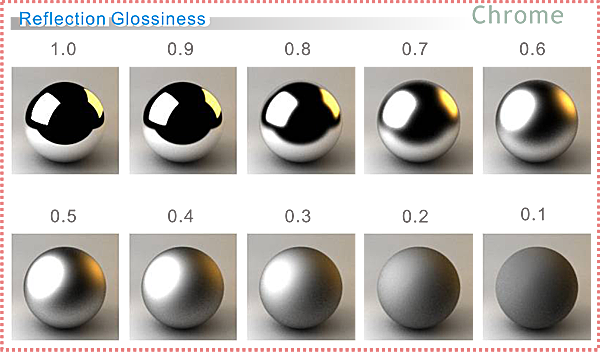
\includegraphics[width=0.8\textwidth]{reflection_layer_in_vray_for_sketchup_4.png}
    \caption{Glossiness and its change on reflection as shown in raytracing software. Source: Online \citet{gloss15}}
    \label{fig:reflection_layer_in_vray_for_sketchup_4}
\end{figure}
\FloatBarrier

\subsection{Computing platform}
The processing of images may be done by humans, in which the image is sent directly to a screen. In cases where we want to use machine vision algorithms, a general purpose computer is typically doing this job.

The computing platform is connected to the camera, and it gathers images which is then processed by a computer program.

Computer performance using a central processing unit is steadily increasing as new technologies evolve, but a relatively new method uses a graphical processing unit to accelerate application code. This allows for highly parallel execution of code, that may for some algorithms, speed up their execution and in turn speed up the program.

\subsection{Threading}
In order to allow several different threads to run simultaneously, the operating system supports threads. It is also possible to delegate a thread to a specific computing core in a central processing unit, if there are more. This have both advantages and disadvantages.

Advantages include the ability for the computer to use idle processing time, and also allow for blocking functions to run in seperate threads to allow the main thread to continue running.

Disadvantages include possibilities of interfering with each other if they share memory, and it is also notoriously challenging to write good multi threaded applications, which in turn may lead to the program not functioning as expected.

In the case of video compression, some codecs are more suited for parallel computing, while others are not. If one is intending to compress video, this should  be kept in mind so that a codec that supports parallel computing is selected. The codec may also use the GPU for speedups.

\begin{figure}[ht]
    \centering
    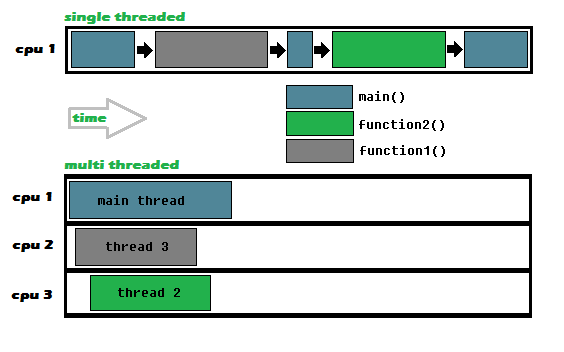
\includegraphics[width=1.0\textwidth]{multithreading.png}
    \caption{Singlethread versus multithread execution. Source: Online \citet{multithreadingcpp15}}
    \label{fig:multithreading}
\end{figure}
\FloatBarrier

Modern central processing units contains several computing cores, which can run their own threads if the programmer wishes. The number of computing cores usually range from one to eight in personal computers.

\subsection{Heterogenous computing}
Systems that utilize dissimilar processing cores are known as heterogenous computing systems. Not only do they have the benefit of several processing cores, they also bring the benefit of having dissimilar processing units that work differently and are better at handling specific tasks.

Heterogenous System Architecture can be used to integrate central processing units and graphical processing units, the alternative is to use a parallel computing platform like OpenCL or CUDA that relieves the programmer from having to move data between the processing units themselves.

\begin{figure}[ht]
    \centering
    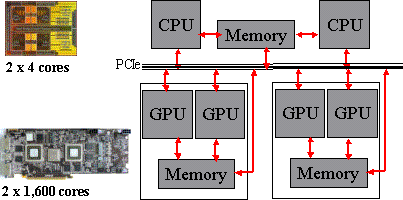
\includegraphics[width=0.8\textwidth]{cpu-gpu.png}
    \caption{Conceptual overview of a heterogeneous system with CPU and GPU cores. Source: Online \citet{cpugpu13}}
    \label{fig:cpu-gpu.png}
\end{figure}
\FloatBarrier

\subsubsection{CUDA}
The NVIDIA Corporation released the CUDA platform in June 2007, and is a parallel computing platform that only works with NVIDIA graphic cards. Language bindings exist for many programming languages, and it provides both low-level and high-level APIs.

\begin{figure}[ht]
    \centering
    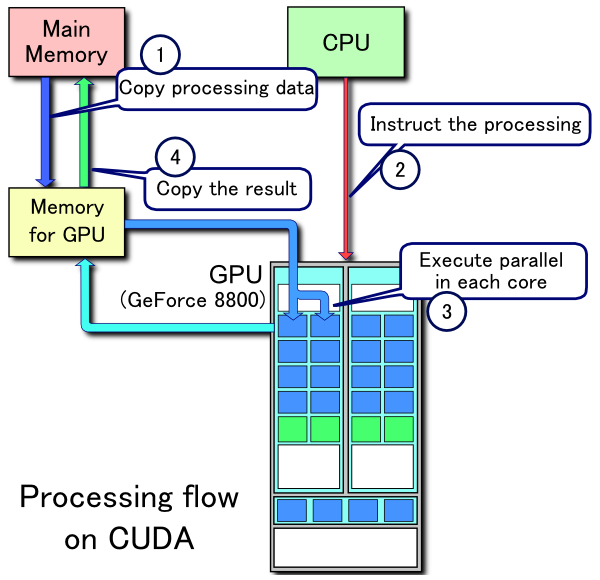
\includegraphics[width=0.8\textwidth]{CUDA_processing_flow_(En).PNG}
    \caption{CUDA processing flow. Source: Online \citet{wikicuda15}}
    \label{fig:CUDA_processing_flow_(En)}
\end{figure}
\FloatBarrier

\subsubsection{OpenCL}
Apple Inc. authored a language and an API that executes across central processing units, graphical processing units and other processors in August 2009. This is now maintained by the Khronos Group, which is a non-profit consortium that develops open standards for graphics, media and parallel computation. They also maintain OpenGL, which sees great use in 3D applications.

OpenCL sees all computing devices, not only the graphical processing units, and a key feature of it is to be portable and run on any system that conforms to the standard.

A comprehensive study by \citep{fang11} in 2011 compared CUDA to OpenCL, and the findings suggests that CUDA performs 30 percent faster than OpenCL when a program is directly translated between the two platforms. However, the conclusion is that there are no reason for OpenCL to perform worse than CUDA under a fair comparison, and OpenCL is considered a good alternative to CUDA.

\subsection{Machine vision}
Machine vision is a relatively new field that uses image capture and analysis for automating tasks. It sees wide use in industrial manufacturing for quality control and process automation, and also in more recent times, autonomous vehicles.

Implementing machine vision in software is often done by using vision libraries, and one well-known is the Open Source Computer Vision Library. The short-form is OpenCV, and it is currently on its third release, being maintained by a russian company named Itseez and developed by contributors all around the world.

OpenCV 3.0 gold release was made available in 4th of June 2015. It supports OpenCL using its transparent API, and support for CUDA was developed in 2010. Both the OpenCL and CUDA support is still under active development.

Performance speedups of groups of algorithms by using GPU acceleration with CUDA can be seen in figure \ref{fig:perfcudavscpuopencv}, tests done by the OpenCV project.

\begin{figure}[ht]
    \centering
    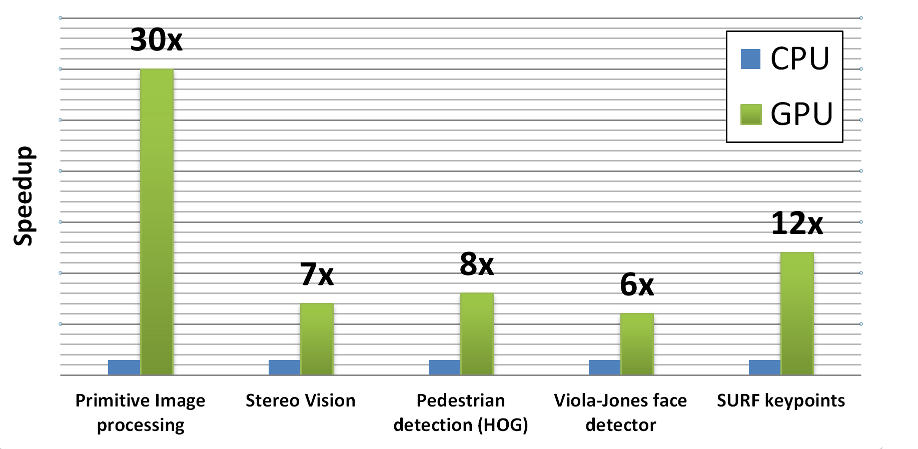
\includegraphics[width=0.8\textwidth]{perfcudavscpuopencv.png}
    \caption{Performance speedups when using CUDA and a GPU. Source: Online \citet{opencvcuda15}}
    \label{fig:perfcudavscpuopencv}
\end{figure}
\FloatBarrier

\subsection{Computer vision}
Computer vision is a field with overlaps from machine vision. Computer vision concerns automatic extraction, analysis and understanding of useful information. Computer vision is also used for visual computer programs that displays data.

\paragraph{Author's comments}
The usage of "computer vision" and "machine vision" is often intermixed, and the exact definition of each is unknown. For the purpose of this thesis, the assumption is that when someone mentions one of these terms, the other may be the one they were meaning to use.

\begin{figure}[ht]
    \centering
    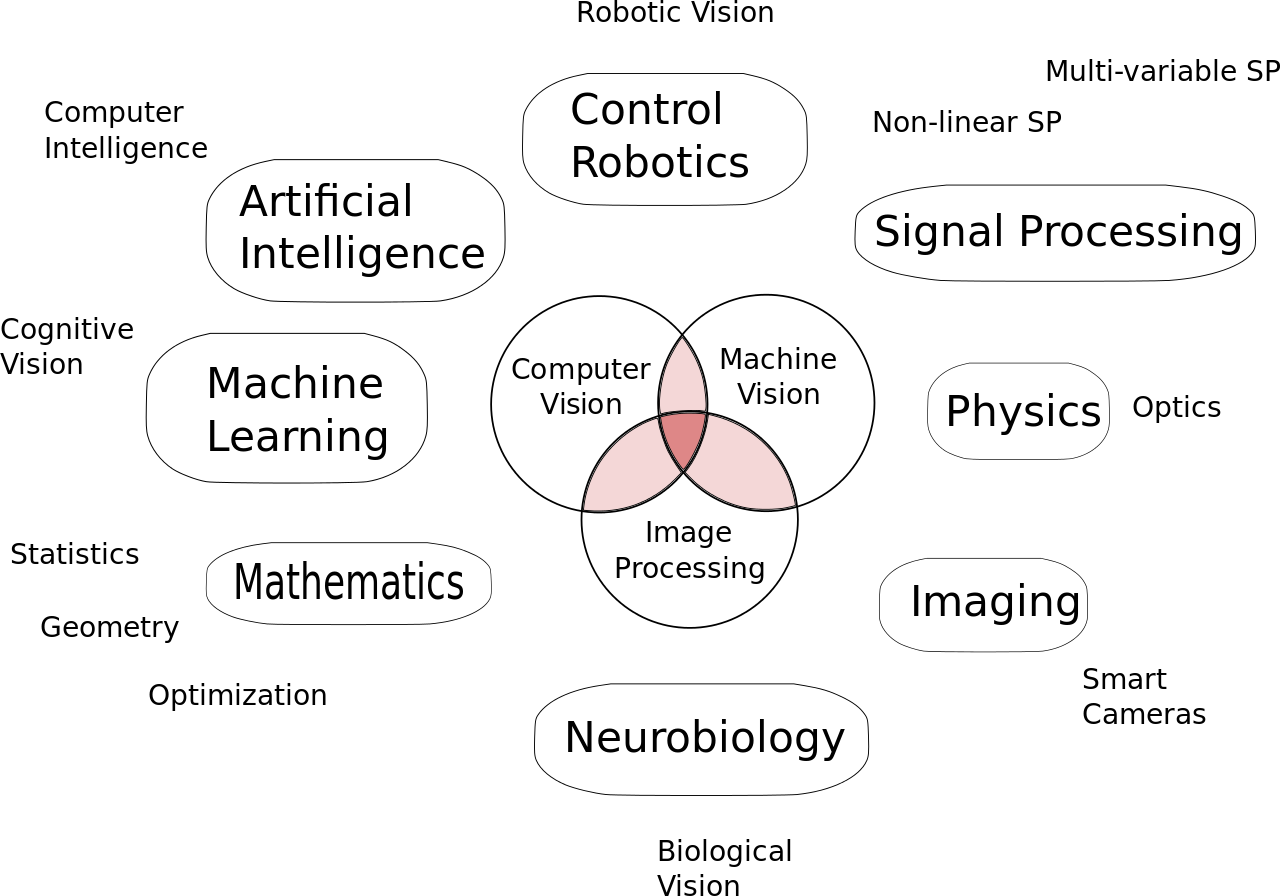
\includegraphics[width=0.8\textwidth]{cvmvwiki.png}
    \caption{Relation between computer vision and various other fields, including machine vision. Source: Online \citet{cvmvwiki15}}
    \label{fig:cvmvwiki}
\end{figure}
\FloatBarrier

\subsection{Linux}
An alternative to Microsoft Windows, the operating system that can run on the widest range of computer architectures is Linux. The operating system kernel was first released in 1991 by Linus Torvalds, and it is a clone of UNIX.
It is a free and open-source collaboration, being developed by programmers all around the world.
The great power of Linux comes through its flexibility, and it or a flavor of it is commonly found powering the servers that make up the world wide web.
Every flavor of Linux is known as a distribution, and most of the larger distributions come with great package management tools.
For Ubuntu, we can use the same tools as are used in the Debian distribution, which includes apt-get, to install the latest releases of open source software.
It is possible to optimize software running on a Linux system further than what is possible with a Microsoft Windows system, and there is by default less overhead on Linux.
Some downsides of using Linux include a very fragmented software world, and many bleeding edge updates that can make the system stop working if carelessly updated. The learning curve is also steeper, and a lot of frustration is to be expected if one has not worked with Linux before.
A great resource to learn more about the Linux operating system is Wikipedia \citep{wikiLinux15} and Linus Torvalds GitHub-repository for Linux \citep{githubLinux15}.

